% Chapter 2

\chapter{Propuesta tecnol\'ogica} % Main chapter title

\label{Chapter3} % For referencing the chapter elsewhere, use \ref{Chapter1} 

%----------------------------------------------------------------------------------------

% Define some commands to keep the formatting separated from the content 

%----------------------------------------------------------------------------------------
Dada la introducci\'on correspondiente, en este cap\'itulo se describe la
propuesta tecnol\'ogica que compete a este proyecto, para esto se propone, en
particular, articular una soluci\'on que se identifique en el \'area de las
\emph{smart wheelchair} 
\section{Silla de ruedas inteligente}
Una silla de ruedas inteligente \emph{smart} es cualquier silla auto propulsada
que utiliza un sistema de contro para aumentar o incluso reemplazar el control
del usuario \parencite{smart}. Su prop\'osito es el de reducir o eliminar las
acciones del usuario para conducir la silla. Usualmente, una silla de ruedas
inteligente es controlada v\'ia una computadora, tiene una colecci\'on de
sensores y aplica t\'ecnicas de mobilidad de la rob\'otica, pero todo esto no es
exclusivamente necesario. La interfaz puede consistir de un joystick tradicional
de silla de ruedas, un dispositivo \emph{sip-and-puff} \footnote{tecnolog\'ia
que mediante inalaciones el usuario puede utilizar para indicar acciones}, o
alguna pantalla sensible al tacto. Estas en particular difieren de cualquier
otra silla de ruedas motorizada en el sentido en que, en estas \'ultimas el
usuario es quien controla la velocidad y direcci\'on del veh\'iculo por
completo, en una \emph{smart wheelchair} esta tarea es apoyada por el sistema de
control de la misma.\\
Las sillas de ruedas inteligentes son dise\~nadas para una gran variedad de
tipos de usuarios. Algunas son dise\~nadas para usuarios con deficiencias
cognitivas, como la demencia, estas comunmente son acondicionadas con sistemas y
t\'ecnicas de evaci\'on de colisiones logrando que incluso aunque el usuario lo
indique, estas no incurran en una situaci\'on de choque que pueda lastimar al
usuario. Algunas otras se enfocan en servir a pacientes con severas
discapacidades motoras, como la par\'alisis cerebral y/o la cuadraplejia y el
roll de la silla de ruedas es el de interpretar peque\~nas activaciones
musculares como comandos de alto nivel y ejecutarlos. Estas sillas por lo
general emplean t\'ecnicas de la inteligencia artificial, como la planeaci\'on
de trayectorias.

\section{Componentes}

\tikzstyle{block} = [draw, fill=blue!20, rectangle, 
    minimum height=3em, minimum width=6em]
\tikzstyle{sum} = [draw, fill=blue!20, circle, node distance=2cm]
\tikzstyle{input} = [coordinate]
\tikzstyle{output} = [coordinate]
\tikzstyle{pinstyle} = [pin edge={to-,thin,black}]

\begin{figure}
    \centering
% The block diagram code is probably more verbose than necessary
\begin{tikzpicture}[auto, node distance=3cm,>=latex']
    % We start by placing the blocks
    \node [input, name=input] {};
    \node [block, right of=input] (interfaz) {Intefaz};
    \node [sum, right of=interfaz] (sum) {};
    \node [block, right of=sum] (controlador) {Control};
    \node [block, right of=controlador] (power) {Potencia};
    \node [block, below of=controlador] (measurements) {Sensores};
    % We draw an edge between the controller and system block to 
    % calculate the coordinate u. We need it to place the measurement block. 
    \node [output, right of=power] (output) {};

    % Once the nodes are placed, connecting them is easy. 
    \draw [draw,->] (input) -- node {usuario} (interfaz);
    \draw [->] (interfaz) -- node {} (sum);
    \draw [->] (sum) -- node {} (controlador);
    \draw [->] (controlador) -- node {} (power);
    \draw [->] (power) -- node [name=y] {carga}(output);
    \draw [->] (y) |- (measurements);
    \draw [->] (measurements) -| node[pos=0.99] {$+$} 
        node [near end] {} (sum); 
\end{tikzpicture}
\caption{Definici\'on esquem\'atica de la soluci\'on}
\label{fig:esquemas}
\end{figure}


Como se muestra en la figura \ref{fig:esquemas} se proponen los siguientes
componentes para la composici\'on final de la soluci\'on:
\begin{itemize}
    \item Interfaz de usuario
    \item Sistema de control
    \item Sistema de potencia
    \item Sensores
\end{itemize}

\subsection{Esquema f\'isico}

\begin{figure}[th]
    \centering
    \includegraphics[width=.8\textwidth]{Figures/whelchair.jpg}
    \decoRule
    \caption{Silla de ruedas tradicional y manual}
    \label{fig:manual}
\end{figure}

Adem\'as de que, los componentes antes mencionados ser\'an descritos a
profundidad en las siguientes secciones, cabe aclarar que, como parte de la
propuesta de soluci\'on, se plantea el hecho de que dichos sistemas ser\'an
integrados sobre una silla de ruedas tradicional. ref.\ref{fig:manual}

Siendo as\'i podemos catalogar en este momento a esta propuesta como un
\emph{upgrade} m\'as que como un producto nuevo, a\'un as\'i como es descrito en
el cap\'itulo \ref{Chapter2} existe una necesidad real en el mercado por una
alternativa m\'as sofisticada en sectores de la sociedad no tan favorecidos.

\section{Interf\'az de usuario}

\begin{figure}[th]
    \centering
    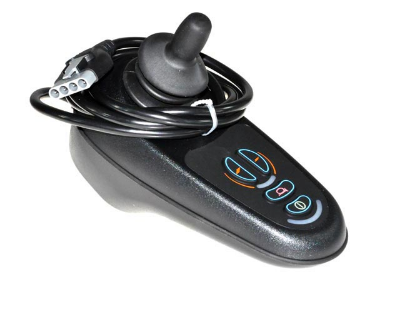
\includegraphics[width=.4\textwidth]{Figures/joystick.png}
    \decoRule
    \caption{Joystick tradicional}
    \label{fig:joystick}
\end{figure}
En este apartado se opta por ir con un sistema tradicional, dado que seg\'un las
observaciones del mercado que se hicieron en el ca\'pitulo \ref{Chapter2},
existe una gran demanda en el sector de los usuarios de sillas de ruedas con
capacidad motriz para operar un \emph{joystick} y aunado a la generosa oferta en
el mercado de dispositivos de este estilo, esto es determinado.\\



\section{Sistema de control}

Se propone un sistema de control autom\'atico para la \emph{silla smart} este
tendr\'a las siguientes tareas:
\begin{itemize}
    \item Procesar la se\~nal proveniente del joystick de control
    \item Interpretar las distintas se\~nales provenientes de los sensores
    \item Generar la salida adecuada para el sistema de potencia
\end{itemize}

Una de las consideraciones al momento de desarrollar dicho sistema de control es
que: \textbf{el usuario final ser\'a quien dirija la silla de ruedas} pero \textbf{el
sistema de control de la silla asistir\'a dicha conducci\'on.}\\

Con lo anterior planteado el sistema de control propuesto tendr\'a una tarea
bastante delimitada y se propone que resida en una computadora a bordo, el
detalle de su implementaci\'on se discute en el siguiente cap\'itulo.


\section{Sistema de potencia}

\subsection{Almacenamiento}

\begin{figure}[th]
    \centering
    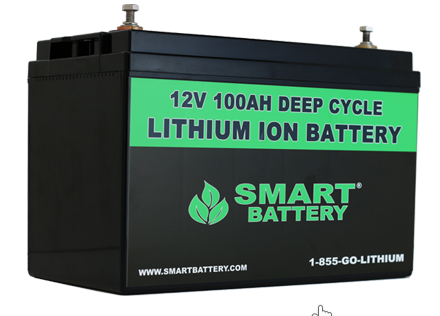
\includegraphics[width=.4\textwidth]{Figures/batery.png}
    \decoRule
    \caption{Banco de baterias; $12v$}
    \label{fig:batery}
\end{figure}

Para satisfacer a todo el sistema de energ\'ia se propone el uso de bater\'ias
el\'ectricas abordo. Dada la informaci\'on expuesta en el cap\'itulo
\ref{Chapter1} se elige el uso de las bater\'ias que entregar\'an una mejor
relaci\'on de densidad energ\'etica: las bater\'ias de iones de litio.\\
Dado que es un est\'andar en las sillas de ruedas motorizadas el uso de dos
bancos de baterias de $12v$ cada una, en este caso se opta por seguir con dicha
tendencia

\subsection{Entrega de potencia}

\begin{figure}[th]
    \centering
    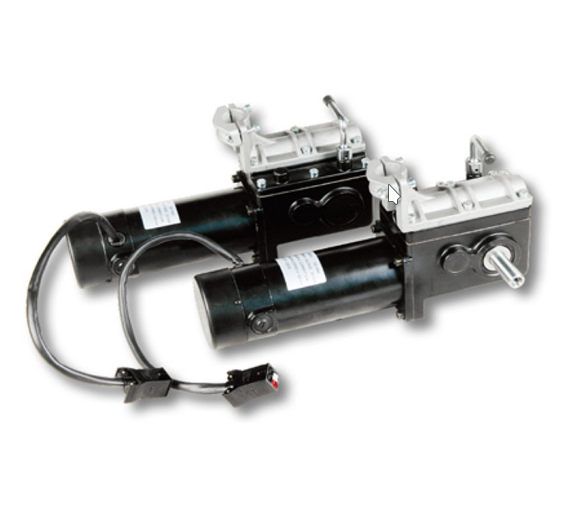
\includegraphics[width=.5\textwidth]{Figures/motor.png}
    \decoRule
    \caption{Par de motores de DC}
    \label{fig:motor}
\end{figure}

Para la entrega de potencia a la silla se utilizar\'an un par de motores de
corriente directa (fig.\ref{fig:motor}) acoplados sobre un chasis debajo del asiento de la silla
tradicional y directamente conectados a las ruedas estos contar\'an tambien con
un par de encoders \'opticos y el correspondiente controlador, mismos en los que
se aunar\'a en su descripci\'on en el siguiente cap\'itulo

\section{Sensores}

Con la intenci\'on de dotar al sistema de una retroalimentaci\'on que permita al
usuario final una experiencia de conducci\'on m\'as rica y sencilla, se pretende
incorporar en la soluci\'on distintos sensores, entre los que se encuentran,
pero no exclusivamente:
\begin{itemize}
    \item Sensores ultras\'onicos
    \item Sensores de nivel de bateria
    \item Aceler\'ometros
    \item Girosc\'opios
    \item Sensores de presi\'on
\end{itemize}
